\documentclass{article}
\usepackage[en]{homework}
\usepackage{tikz}
\usepackage{needspace}
\usetikzlibrary{arrows.meta,calc}

\definecolor{diagramaccent}{RGB}{43,83,124}
\tikzset{
  homework diagram/.style={
    text=black, line width=.7pt, line cap=round, line join=round,
    >={Stealth[length=2.2mm,width=1.5mm]}, font=\normalfont\small
  },
  diagram dashed/.style={dash pattern=on 3pt off 2pt},
  diagram orbit/.style={draw=black!75, line width=.7pt},
  diagram trajectory/.style={draw=diagramaccent, line width=.9pt},
  diagram vector/.style={draw=diagramaccent, line width=.9pt, ->},
  diagram guide/.style={draw=black!55, line width=.45pt},
  diagram dimension/.style={
    diagram guide, <->, >={Stealth[length=1.6mm,width=1.1mm]}
  },
  diagram body/.style={draw=black!75, fill=black!8, line width=.7pt},
  diagram point/.style={draw=black!75, fill=shadecolor, line width=.7pt}
}

\config{Physics-1}{2026 Fall}{7}

\begin{document}

\begin{problem}
A rocket is fired straight up through the atmosphere from the South Pole, burning out at an altitude of $250\ \mathrm{km}$ when traveling at $6.00\ \mathrm{km/s}$.
\begin{enumerate}
  \item[(a)] What maximum distance from the Earth's surface does it travel before falling back to the Earth?
  \item[(b)] Would its maximum distance from the surface be larger if the same rocket were fired with the same fuel load from a launch site on the equator? Why or why not?
\end{enumerate}
\end{problem}

\begin{solution}
	\paragraph{(a)} Denote the mass and the radius of the Earth by $M_E$ and $R_E$ respectively, and the altitude and speed of the rocket when it burns out by $h_0 = 250\ \mathrm{km}$ and $v_0 = 6.00\ \mathrm{km/s}$. According to the conservation of energy, when the rocket reaches the highest altitude $h_{\mathrm{max}}$,
	\[ \frac{1}{2}m v_0^2 - \frac{GM_E m}{R_E + h_0} = -\frac{GM_E m}{R_E + h_{\mathrm{max}}}. \]
	Canceling $m$ and using $R_E = 6.37\times 10^6\ \mathrm{m}$ and $GM_E = 3.986\times 10^{14}\ \mathrm{m^3/s^2}$, we obtain
	\[ h_{\mathrm{max}} = \left(\frac{1}{R_E+h_0}-\frac{v_0^2}{2GM_E}\right)^{-1}-R_E
	\approx 3.07\times 10^6\ \mathrm{m} = 3.07\times 10^3\ \mathrm{km}. \]

	\paragraph{(b)} Yes. Because the rotation of the Earth can give the rocket more initial kinetic energy when launching.
\end{solution}



\begin{problem}
Two stars of masses $M$ and $m$, separated by a distance $d$, revolve in circular orbits about their center of mass. Obtain the period of each of the stars.
\begin{center}
  % AI-assisted redraw of the supplied binary-star diagram.
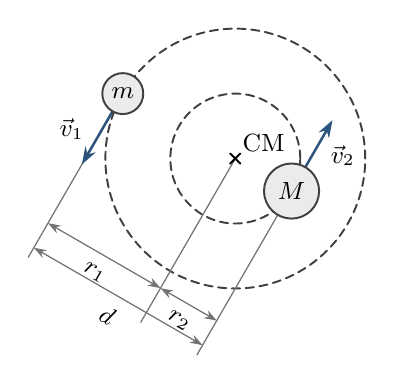
\begin{tikzpicture}[homework diagram]
  \coordinate (O) at (0,0);
  \coordinate (m) at (150:1.65);
  \coordinate (M) at (330:.825);
  \coordinate (md) at ($(m)+(-.95,-1.6454)$);
  \coordinate (Od) at (-.95,-1.6454);
  \coordinate (Md) at ($(M)+(-.95,-1.6454)$);

  \draw[diagram orbit, diagram dashed] (O) circle[radius=1.65];
  \draw[diagram orbit, diagram dashed] (O) circle[radius=.825];
  \draw[diagram guide] (m) -- ($(md)+(-.25,-.433)$);
  \draw[diagram guide] (O) -- ($(Od)+(-.25,-.433)$);
  \draw[diagram guide] (M) -- ($(Md)+(-.25,-.433)$);
  \draw[diagram dimension] (md) -- node[below=1pt, sloped] {$r_1$} (Od);
  \draw[diagram dimension] (Od) -- node[below=1pt, sloped] {$r_2$} (Md);
  \draw[diagram dimension] ($(md)+(-.18,-.312)$)
    -- node[below=1pt, sloped] {$d$} ($(Md)+(-.18,-.312)$);

  \draw[diagram vector]
    (m) -- ++(-.52,-.90) node[midway, left=3pt] {$\vec{v}_1$};
  \draw[diagram vector]
    (M) -- ++(.52,.90) node[midway, right=3pt] {$\vec{v}_2$};
  \node[diagram body, circle, minimum size=5.2mm, inner sep=0pt] at (m) {$m$};
  \node[diagram body, circle, minimum size=7mm, inner sep=0pt] at (M) {$M$};
  \draw (-.065,-.065) -- (.065,.065)
    (-.065,.065) -- (.065,-.065);
  \node[above right=-1pt] at (O) {CM};
\end{tikzpicture}

\end{center}
\end{problem}

\begin{solution}
	Suppose the system is rotating with angular speed $\omega$. The gravitational force between two stars is given by 
	\[ F = \frac{GMm}{d^2}. \]
	Therefore, from the formula of circular motion, 
	\[ F = mr_1\omega^2 = Mr_2\omega^2. \]
	Since $r_1+r_2=d$ and the center-of-mass condition gives $mr_1=Mr_2$, we have
	\[ r_1 = \frac{M}{M+m}d, \qquad r_2 = \frac{m}{M+m}d. \]
	Substituting $r_1$ into the force equation gives
	\[ \omega^2 = \frac{F}{mr_1}
	= \frac{GMm}{d^2}\frac{M+m}{mMd}
	= \frac{G(M+m)}{d^3}. \]
	Both stars have the same angular speed $\omega=\sqrt{G(M+m)/d^3}$, so their periods are equal:
	\[ T_m = T_M = T = \frac{2\pi}{\omega}
	= 2\pi\sqrt{\frac{d^3}{G(M+m)}}. \]
\end{solution}



\begin{problem}
\textbf{Projectile rise}

A projectile of mass $m$ is fired from the surface of the Earth at an angle $\alpha$ from the vertical. The initial speed $v_0$ is equal to $\sqrt{GM_E/R_E}$. How high does the projectile rise? Neglect air resistance and the Earth's rotation.
\begin{center}
  % AI-assisted redraw of the supplied projectile diagram.
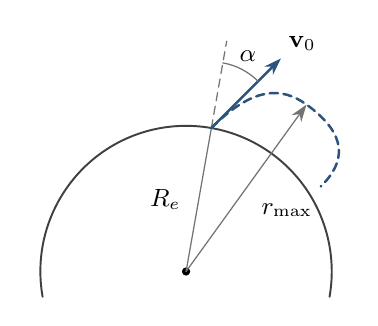
\begin{tikzpicture}[homework diagram]
  \coordinate (O) at (0,0);
  \coordinate (S) at (80:1.85);
  \coordinate (A) at (1.53,2.12);

  \draw[diagram orbit] (190:1.85) arc[start angle=190,end angle=-10,radius=1.85];
  \fill (O) circle[radius=1.5pt];
  \draw[diagram guide] (O) -- node[left=3pt] {$R_e$} (S);
  \draw[diagram guide, diagram dashed] (S) -- ++(80:1.12);
  \draw[diagram trajectory, diagram dashed]
    (S) .. controls (.85,2.35) and (1.212,2.3495) .. (A)
    .. controls (2.06,1.7375) and (2.03,1.39) .. (1.71,1.08);
  \draw[diagram guide, ->] (O) -- node[below right=2pt] {$r_{\max}$} (A);
  \draw[diagram vector]
    (S) -- ++(45:1.25) node[above right=-1pt] {$\mathbf{v}_0$};
  \draw[diagram guide] ($(S)+(45:.84)$)
    arc[start angle=45,end angle=80,radius=.84];
  \node at ($(S)+(63:1.02)$) {$\alpha$};
\end{tikzpicture}

\end{center}
\end{problem}

\begin{solution}
	Denote the speed of the projectile at $r_{\max}$ by $v$. Since the velocity is perpendicular to the radius at this point, from the conservation of angular momentum,
	\[ mR_Ev_0\sin\alpha = mr_{\max}v, \qquad v = \frac{R_Ev_0\sin\alpha}{r_{\max}}. \]
	According to the conservation of energy,
	\[ \frac{1}{2}mv_0^2 - \frac{GM_Em}{R_E} = \frac{1}{2}mv^2 - \frac{GM_Em}{r_{\max}}. \]
	Substituting $v$ and $v_0^2=GM_E/R_E$ into the equation gives
	\[ -\frac{GM_E}{2R_E} = \frac{GM_ER_E\sin^2\alpha}{2r_{\max}^2} - \frac{GM_E}{r_{\max}}, \]
	which can be written as
	\[ r_{\max}^2 - 2R_Er_{\max} + R_E^2\sin^2\alpha = 0. \]
	Taking the larger root, we obtain $r_{\max}=R_E(1+\cos\alpha)$. Therefore, the maximum height above the Earth's surface is
	\[ h_{\max} = r_{\max}-R_E = R_E\cos\alpha. \]
\end{solution}



\begin{problem}
Tianwen-1 was launched to the space in July, 2020. The destination was the Mars. An energy-efficient way to accomplish this is through the so-called Hohmann transfer orbit, as shown in the picture. The orbits of the Earth and the Mars can both be viewed as circular orbits. The Hohmann transfer orbit is tangent to the orbit of earth at the perihelion, and tangent to the orbit of Mars at the aphelion.
\begin{enumerate}
  \item[a.] Calculate the energy needed to transfer from earth orbit to the elliptic orbit, and from the elliptic orbit to Mars orbit.
  \item[b.] Calculate the time needed on the transfer orbit
  \item[c.] Calculate the angle between earth and Mars at the launch time. This determines the so called launch window. For example, July to August of 2020 was a launch window.
  \item[d.] A year for the Mars is 687 days (on earth). How often will a launch window appear?
\end{enumerate}
\begin{center}
  % AI-assisted redraw of the supplied Hohmann transfer diagram.
\begin{tikzpicture}[homework diagram]
  \draw[diagram orbit] (0,0) circle[radius=2.30];
  \draw[diagram orbit] (0,0) circle[radius=1.15];
  \draw[diagram trajectory] (-.575,0) ellipse[x radius=1.725,y radius=1.6263];
  \filldraw[diagram body] (0,0) circle[radius=.095];

  \node[above] at (.75,2.23) {Mars orbit};
  \node at (0,-.78) {Earth orbit};

  \draw[diagram vector]
    (1.39,.29) .. controls (1.10,1.36) and (.40,1.80) .. (-.85,1.83);
  \filldraw[diagram point] (124:2.30) circle[radius=.055];
  \node[align=left, anchor=east] at (-1.39,1.95)
    {Mars' position\\at launch};
  \filldraw[diagram point] (-2.30,0) circle[radius=.055];
  \node[align=left, anchor=east] at (-2.42,0)
    {arrival\\at Mars};
  \node at (1.75,-.03) {launch};
  \node at (0,-2.70) {Hohmann transfer trajectory};
\end{tikzpicture}

\end{center}
\end{problem}

\begin{solution}
	Denote the mass of the Sun and the mass of the spacecraft by $M$ and $m$ respectively, and the radii of the Earth's and Mars' circular orbits by $r_1$ and $r_2$ respectively. The semi-major axis of the transfer orbit is $a=(r_1+r_2)/2$.

	\paragraph{(a)} From the formula $E = -GMm/2a$, we obtain
	\begin{gather*}
		\Delta E_1 = \frac{GMm}{2r_1} - \frac{GMm}{r_1+r_2}
		= \frac{GMm(r_2-r_1)}{2r_1(r_1+r_2)}, \\
		\Delta E_2 = \frac{GMm}{r_1+r_2} - \frac{GMm}{2r_2}
		= \frac{GMm(r_2-r_1)}{2r_2(r_1+r_2)}.
	\end{gather*}

	\paragraph{(b)} The period of an object on an orbit with semi-major axis $a$ is given by $T = 2\pi\sqrt{a^3/GM}$. Since the spacecraft travels along half of the transfer orbit, the time needed is
	\[ t = \frac{T}{2} = \pi\sqrt{\frac{a^3}{GM}}
	= \pi\sqrt{\frac{(r_1+r_2)^3}{8GM}}. \]

	\paragraph{(c)} Denote the periods of the Earth and Mars by $T_1$ and $T_2$ respectively. Their angular speeds are
	\[ \omega_1 = \frac{2\pi}{T_1} = \sqrt{\frac{GM}{r_1^3}}, \qquad
	\omega_2 = \frac{2\pi}{T_2} = \sqrt{\frac{GM}{r_2^3}}. \]
	Suppose Mars is ahead of the Earth by an angle $\varphi$ at launch, measured in the direction of revolution. Taking the Earth's position at launch as the angular origin, the spacecraft arrives at angle $\pi$ after time $t$. Therefore, for Mars to be at the same position,
	\[ \varphi + \omega_2 t = \pi. \]
	Substituting $\omega_2$ and $t$ gives
	\[ \varphi = \pi-\omega_2 t
	= \pi\left[1-\left(\frac{r_1+r_2}{2r_2}\right)^{3/2}\right]. \]

	\paragraph{(d)} To have the same angle between the Earth and Mars at the next launch window, the Earth must gain one full revolution relative to Mars. Denote the time between two launch windows by $\tau$. Then
	\[ (\omega_1-\omega_2)\tau = 2\pi, \]
	so
	\[ \tau = \frac{2\pi}{\omega_1-\omega_2}
	= \left(\frac{1}{T_1}-\frac{1}{T_2}\right)^{-1}
	= \frac{T_1T_2}{T_2-T_1}. \]
	Using $T_1\approx365.25\ \mathrm{days}$ and $T_2=687\ \mathrm{days}$, we obtain
	\[ \tau \approx \frac{365.25\times687}{687-365.25}\ \mathrm{days}
	\approx780\ \mathrm{days}\approx2.14\ \mathrm{years}. \]
\end{solution}



\end{document}
